%%%%%%%%%%%%%%%%%%%%%%%%%%%%%%%%%%%%%%%%%%%%%%%%%%%%%%%%%%%%%%%%%%%%%%%%%%%%%%%
% CMSE 492 Final Project Report Template
% Updated with project-specific content for HW08 proposal
%%%%%%%%%%%%%%%%%%%%%%%%%%%%%%%%%%%%%%%%%%%%%%%%%%%%%%%%%%%%%%%%%%%%%%%%%%%%%%%

\documentclass[aps,prl,preprint,groupedaddress]{revtex4-2}

% Essential packages
\usepackage{graphicx}
\usepackage{dcolumn}
\usepackage{bm}
\usepackage{hyperref}
\usepackage{amsmath}
\usepackage{amssymb}
\usepackage{booktabs}
\usepackage{float}
\usepackage{caption}
\usepackage{subcaption}
\usepackage{listings}
\usepackage{xcolor}

\hypersetup{
    colorlinks=true,
    linkcolor=blue,
    filecolor=magenta,
    urlcolor=cyan,
    citecolor=blue,
}

\begin{document}

\title{Predicting League of Legends Match Outcomes from Early-Game Signals}

\author{Liam Sandy}
\email{liam.sandy@msu.edu}
\affiliation{Department of Computational Mathematics, Science and Engineering\\Michigan State University, East Lansing, MI 48824}

\date{\today}

\begin{abstract}
League of Legends is a match-based esport in which competitive momentum swings rapidly during the opening minutes. Broadcasters, analysts, and coaching staffs increasingly seek quantitative tools that forecast eventual winners using only early-game context, enabling richer storytelling and informed strategy calls. This proposal outlines an end-to-end machine learning plan that ingests the publicly available Diamond-tier match log compiled by Riot-affiliated researchers and released on Kaggle. After establishing an 80/20 stratified split and a structured exploratory data analysis pipeline, I benchmark simple and intermediate classifiers that operate on 39 numeric team-aggregate features captured at the ten-minute mark. Preliminary results show that logistic regression improves markedly over a majority-class baseline (test accuracy 0.72, ROC-AUC 0.81), confirming that early economic and objective-control signals contain predictive value. Building on this foundation, I will compare a penalized logistic model, a tuned random forest, and a multilayer perceptron while documenting reproducible preprocessing, validation, and interpretability workflows. The project will culminate in a LaTeX report, reusable code modules, and a stakeholder-friendly presentation demonstrating how data-driven insights can augment competitive League of Legends analysis.
\end{abstract}

\maketitle

\noindent\textbf{GitHub Repository:} \url{https://github.com/liamsandy/cmse492_project}

%%%%%%%%%%%%%%%%%%%%%%%%%%%%%%%%%%%%%%%%%%%%%%%%%%%%%%%%%%%%%%%%%%%%%%%%%%%%%%%
\section{Background and Motivation}
\label{sec:background}
%%%%%%%%%%%%%%%%%%%%%%%%%%%%%%%%%%%%%%%%%%%%%%%%%%%%%%%%%%%%%%%%%%%%%%%%%%%%%%%

League of Legends (LoL) attracts millions of daily players and supports a global professional ecosystem valued in the hundreds of millions of dollars. Competitive matches unfold in real time, placing a premium on analytic tools that can summarize the state of play for casters, coaching staffs, bettors, and broadcast partners. While modern spectator experiences provide abundant raw statistics, human analysts struggle to weight simultaneous signals---gold income, objective control, vision score, and skirmish outcomes---without the aid of statistical modeling.

Recent work on match prediction typically focuses on complete game trajectories or draft-phase hero matchups, leaving a gap for early-game forecasting. Early prediction matters because production teams must decide which matches to highlight, while coaching staffs benefit from immediate feedback on risky objective trades. Moreover, quantified early momentum can enrich player development pipelines by identifying teams that routinely squander leads.

This project aims to build a reproducible machine learning pipeline that predicts the winning side given only the first ten minutes of match data. Machine learning is well suited to this task: supervised classifiers can digest dozens of correlated numeric features and uncover nonlinear interactions that elude heuristic scoring systems. Deliverables include an interpretable model comparison, attribution analyses, and communication artifacts that translate technical findings into actionable insights for esports stakeholders.

%%%%%%%%%%%%%%%%%%%%%%%%%%%%%%%%%%%%%%%%%%%%%%%%%%%%%%%%%%%%%%%%%%%%%%%%%%%%%%%
\section{Data Description}
\label{sec:data}
%%%%%%%%%%%%%%%%%%%%%%%%%%%%%%%%%%%%%%%%%%%%%%%%%%%%%%%%%%%%%%%%%%%%%%%%%%%%%%%

\subsection{Data Origins}
The dataset derives from the ``League of Legends Diamond Ranked Games (10 min)'' collection curated by Riot-affiliated data engineers and distributed on Kaggle \cite{bobby2020lol}. It aggregates 9,879 ranked solo-queue matches played at the Diamond skill tier during the 2020 season. For each match, Riot's telemetry system records team-level statistics sampled at the ten-minute mark, encompassing combat performance, economy, neutral objectives, and vision control. The Kaggle documentation traces the data pipeline back to Riot's match API, ensuring that the measurements mirror the same sources used by official analytics teams.

\subsection{Dataset Characteristics}
\begin{itemize}
    \item Number of samples (rows): 9,879 matches.
    \item Number of features (columns): 39 predictive features after removing the match identifier and the binary target.
    \item Data types: All features are numeric counts, rates, or binary flags aggregated at the team level; the target \texttt{blueWins} is binary.
    \item Target variable: \texttt{blueWins} equals 1 when the Blue side ultimately secures victory.
\end{itemize}

\subsection{Data Quality Analysis}
The raw table contains no missing values, as confirmed by feature-wise missingness rates of zero. Figure~\ref{fig:missingness} visualizes the top features to document this property. The training split retains balanced classes (49.9\% blue wins), so no resampling is required before modeling. Descriptive statistics show that economic differentials (gold and experience) exhibit the largest ranges, often exceeding 6,000 gold in either direction, while objective counts remain in the 0--3 interval.

\subsubsection{Statistical Summary}
Correlations between features and the target reveal that gold and experience advantages drive the strongest signal (absolute correlation \approx 0.51), followed by total gold earned and neutral-objective control. Figure~\ref{fig:distros} compares the marginal distributions of seven high-impact features across win outcomes, highlighting how early dragon, herald, and turret captures skew toward winning teams. Figure~\ref{fig:objective} summarizes objective-control means by outcome, and Figure~\ref{fig:heatmap} presents a correlation heatmap for the top twelve features. Outlier analysis via the interquartile range indicates that fewer than 1.3\% of observations fall outside Tukey fences for key differentials, suggesting that standard scaling suffices for linear models.

\begin{figure}[H]
    \centering
    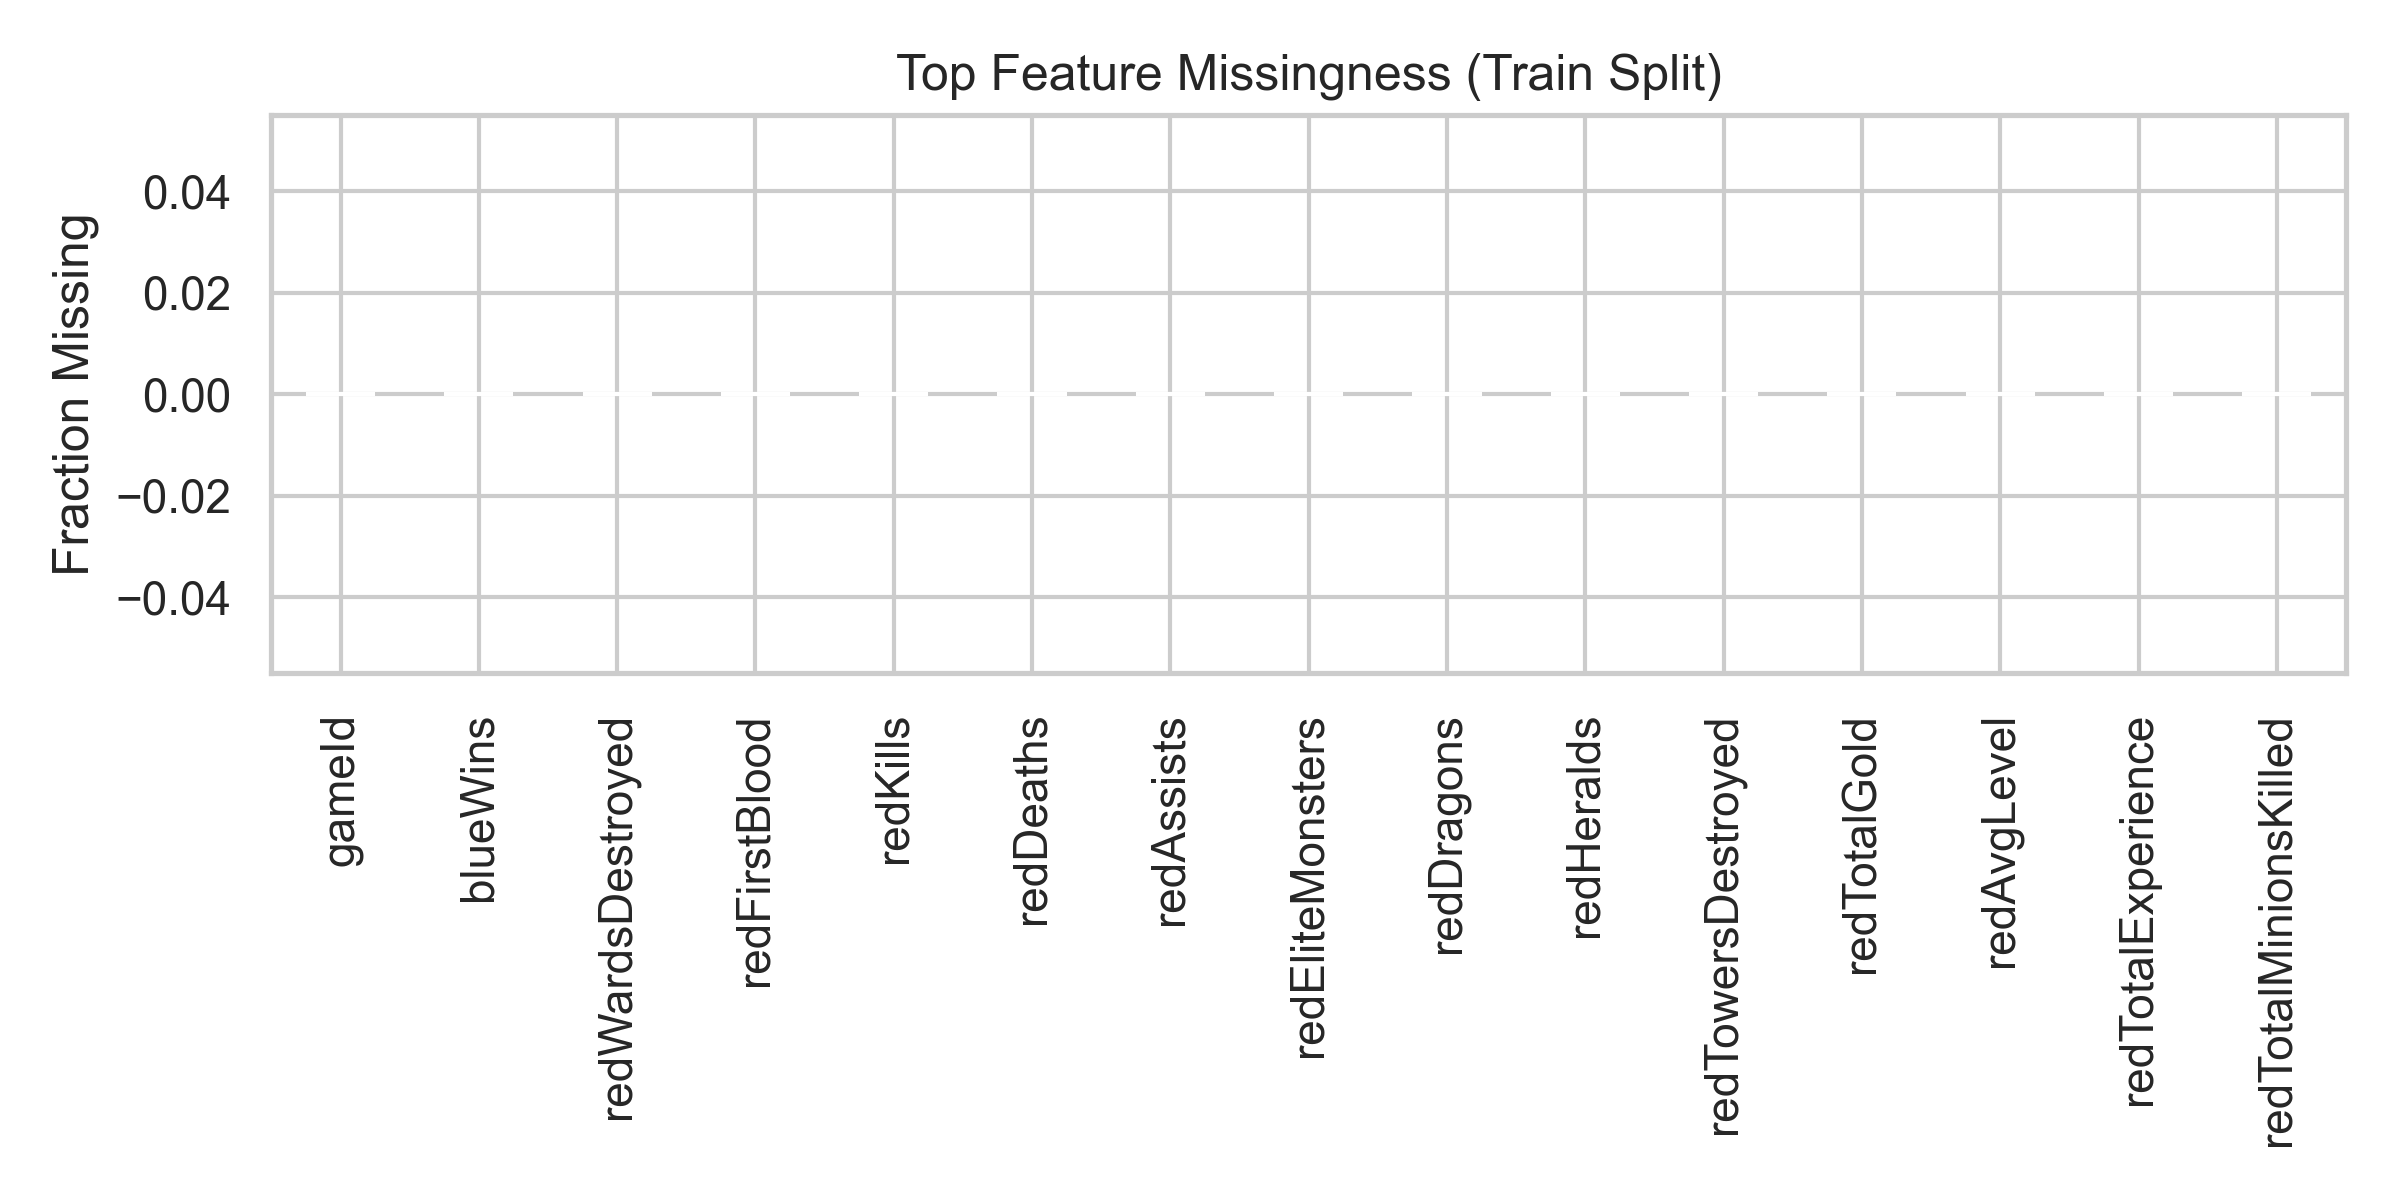
\includegraphics[width=0.7\linewidth]{figures/eda/missingness.png}
    \caption{Feature-level missingness on the training split. All values are zero, confirming complete telemetry coverage.}
    \label{fig:missingness}
\end{figure}

\begin{figure}[H]
    \centering
    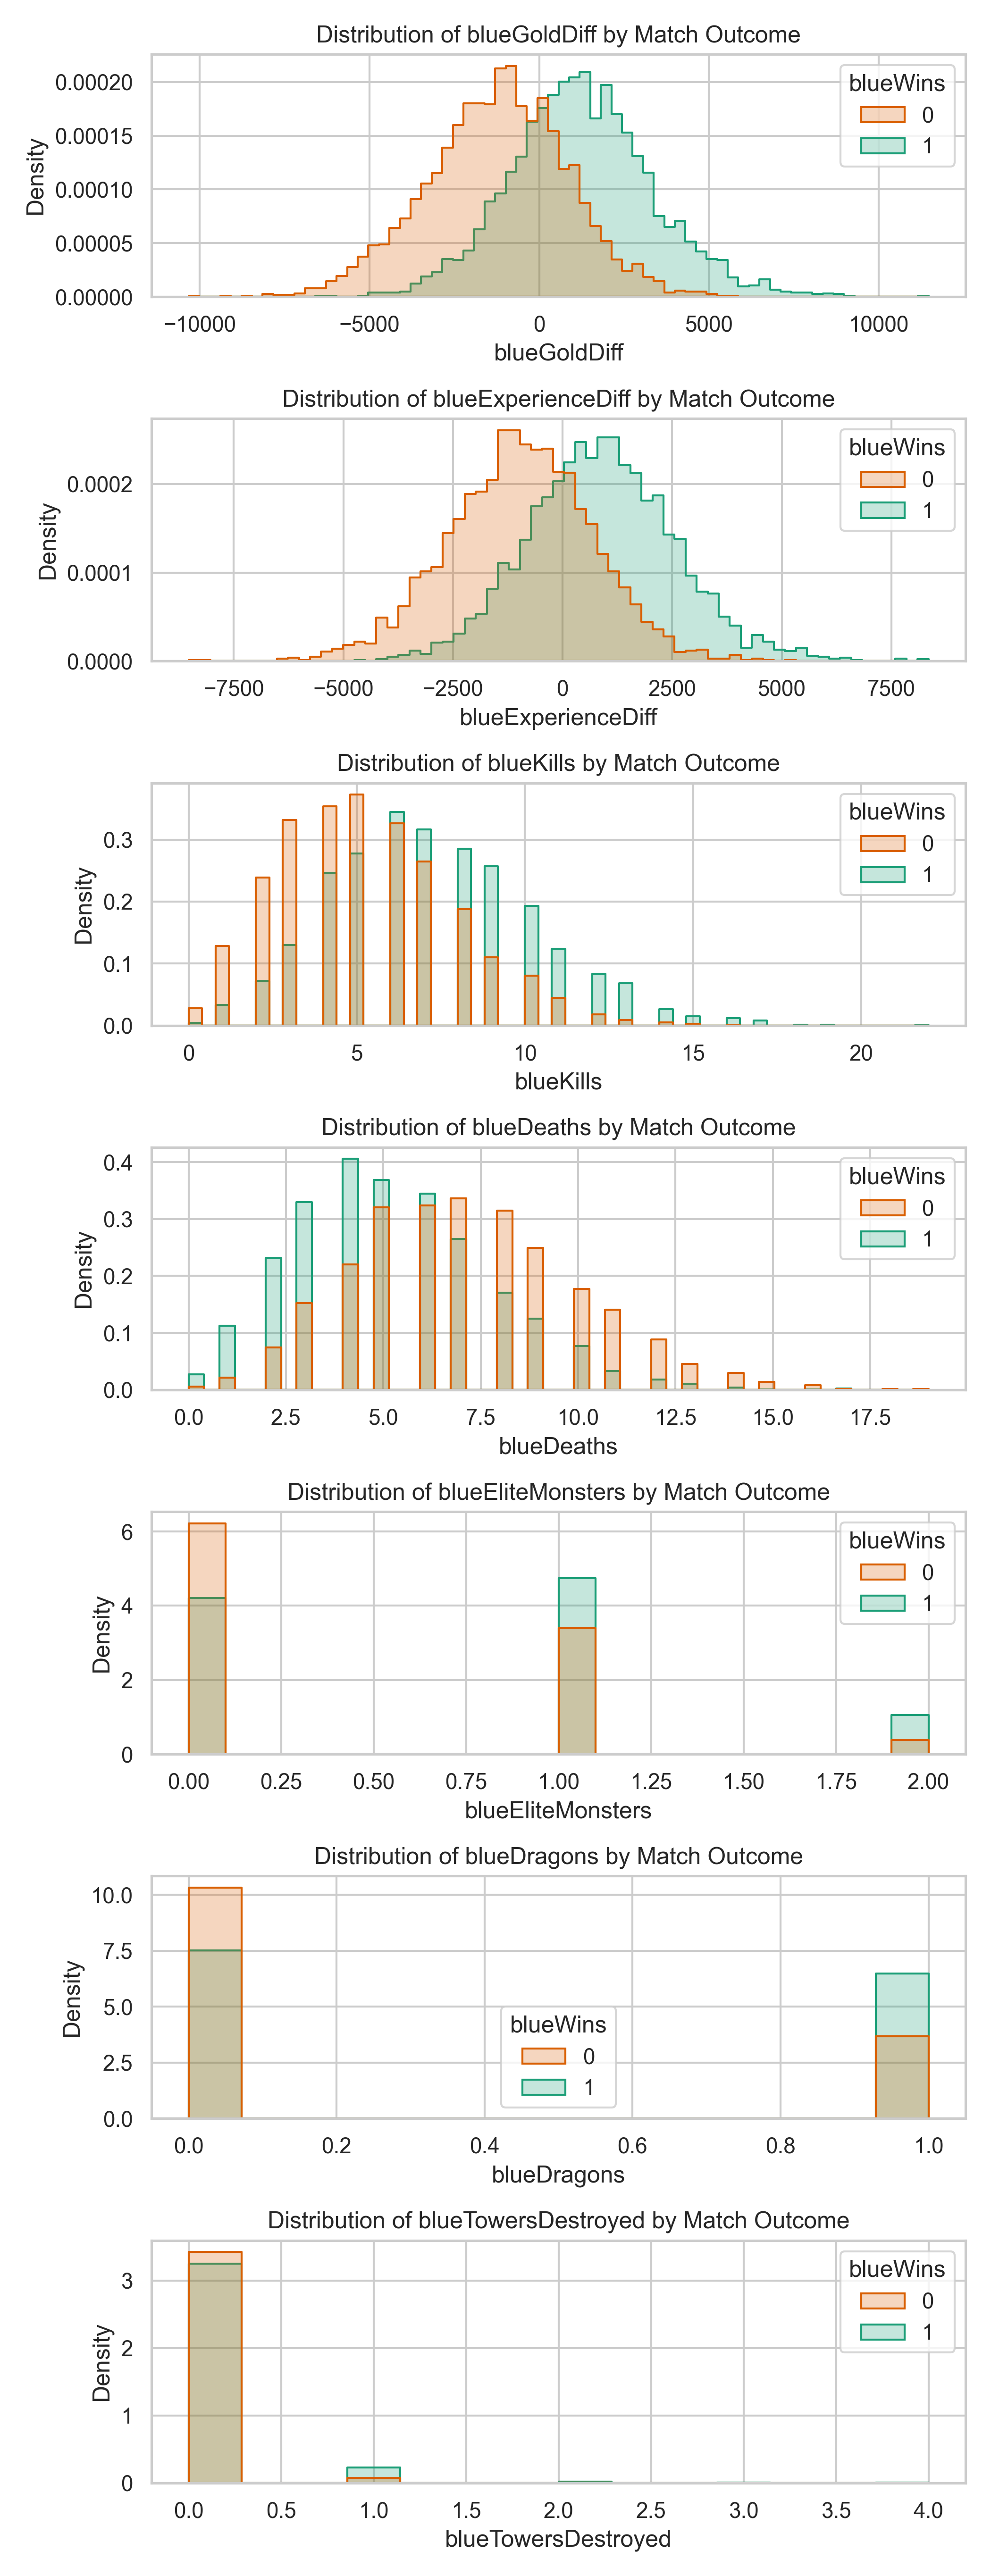
\includegraphics[width=0.72\linewidth]{figures/eda/feature_distributions.png}
    \caption{Outcome-conditioned distributions for high-impact early-game metrics. Winning teams consistently secure superior economic and objective advantages.}
    \label{fig:distros}
\end{figure}

\begin{figure}[H]
    \centering
    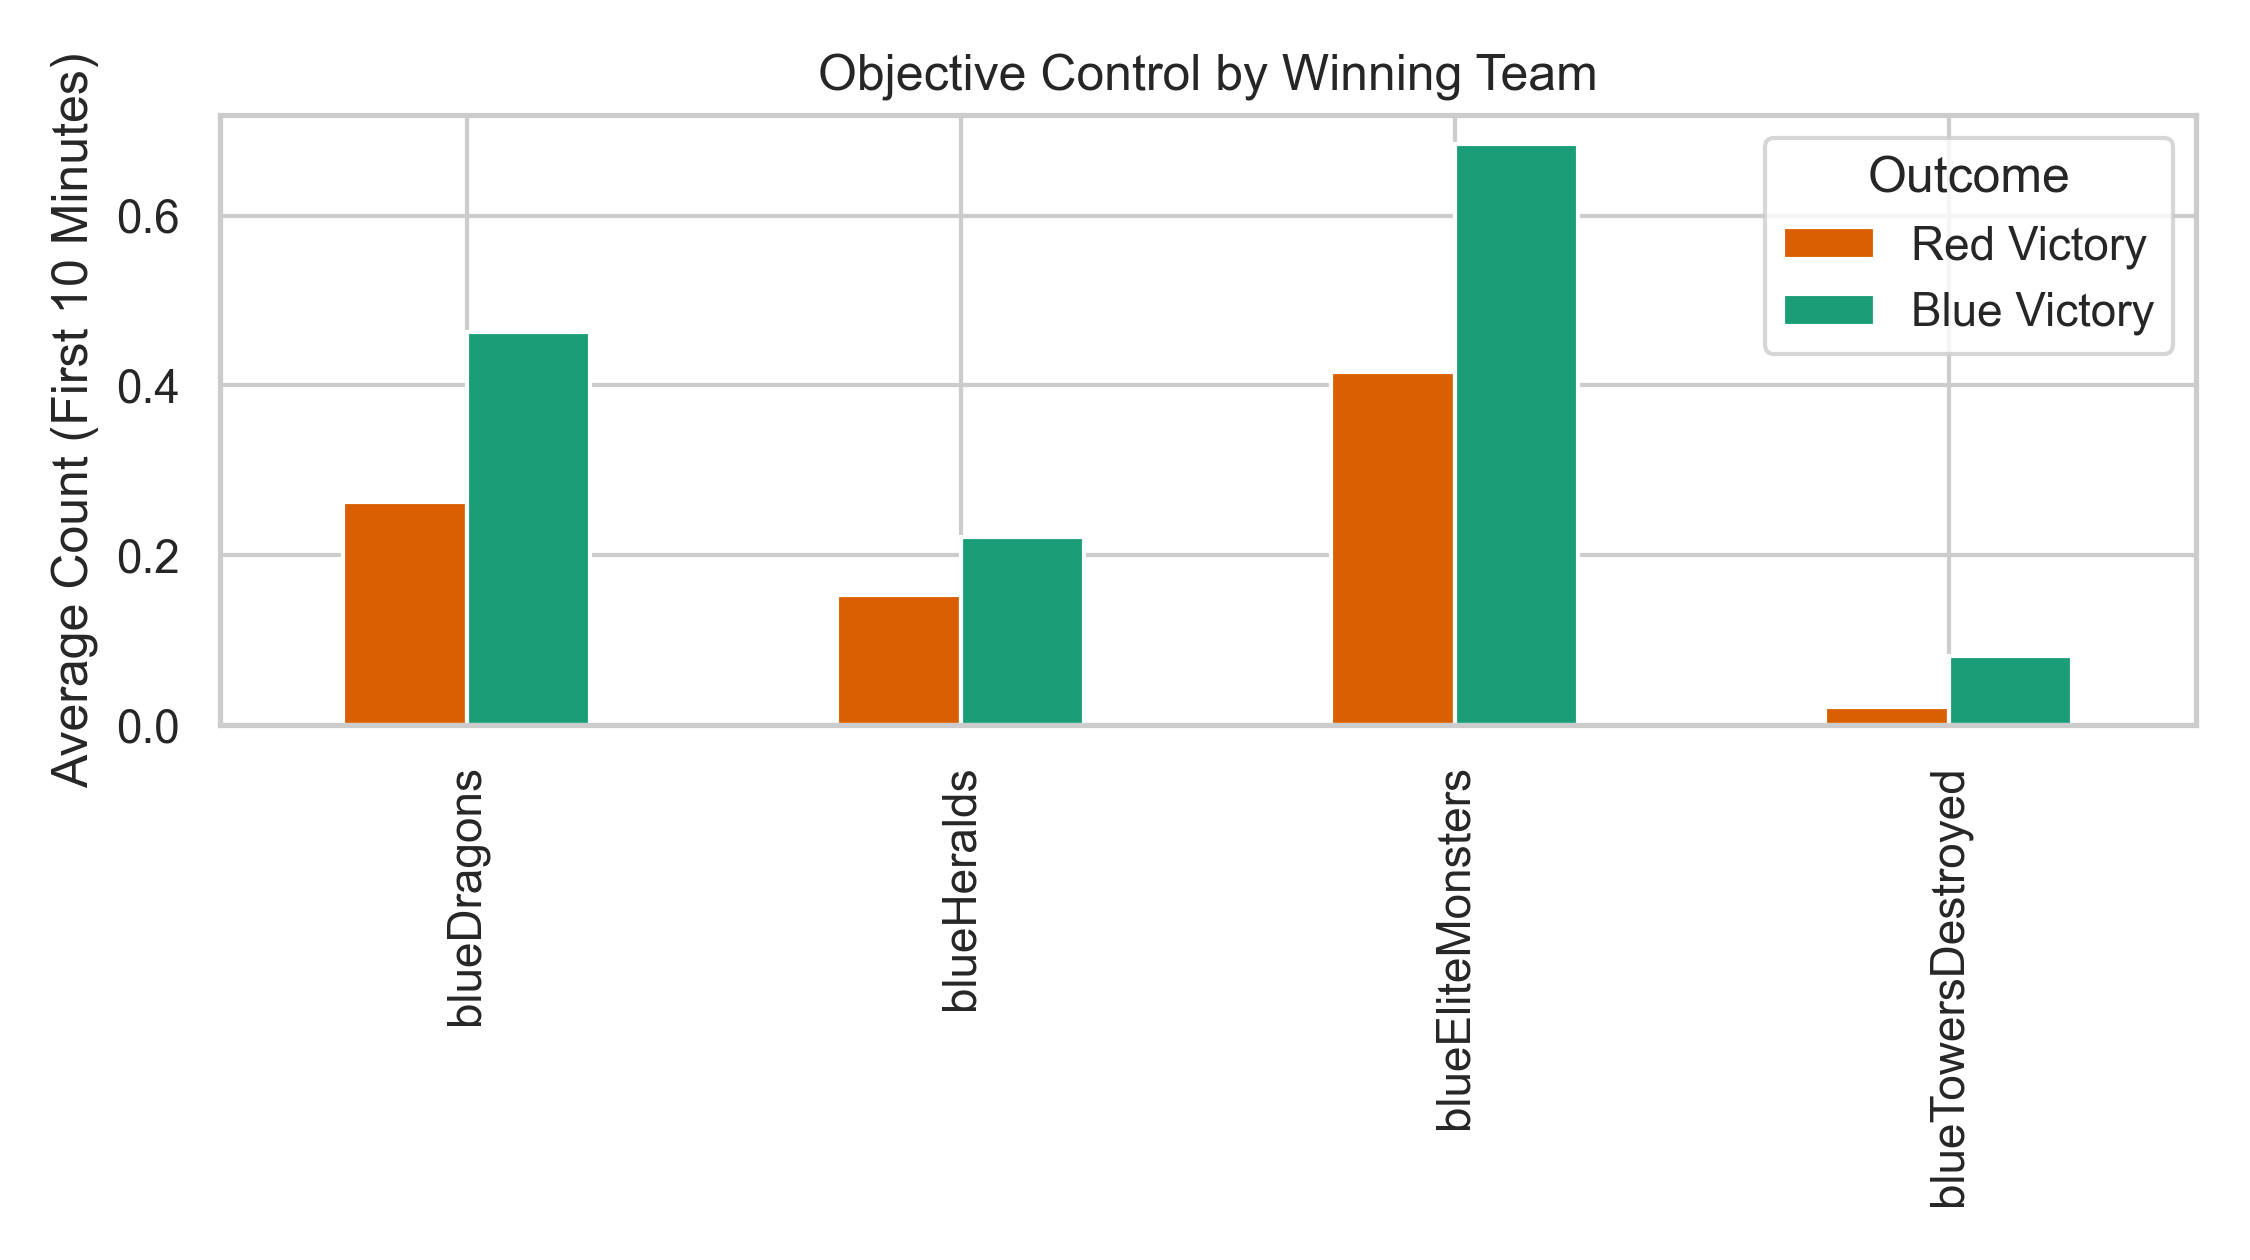
\includegraphics[width=0.65\linewidth]{figures/eda/objective_control.png}
    \caption{Average objective control during the first ten minutes. Blue-side victories correlate with extra dragons, heralds, and turret plates.}
    \label{fig:objective}
\end{figure}

\begin{figure}[H]
    \centering
    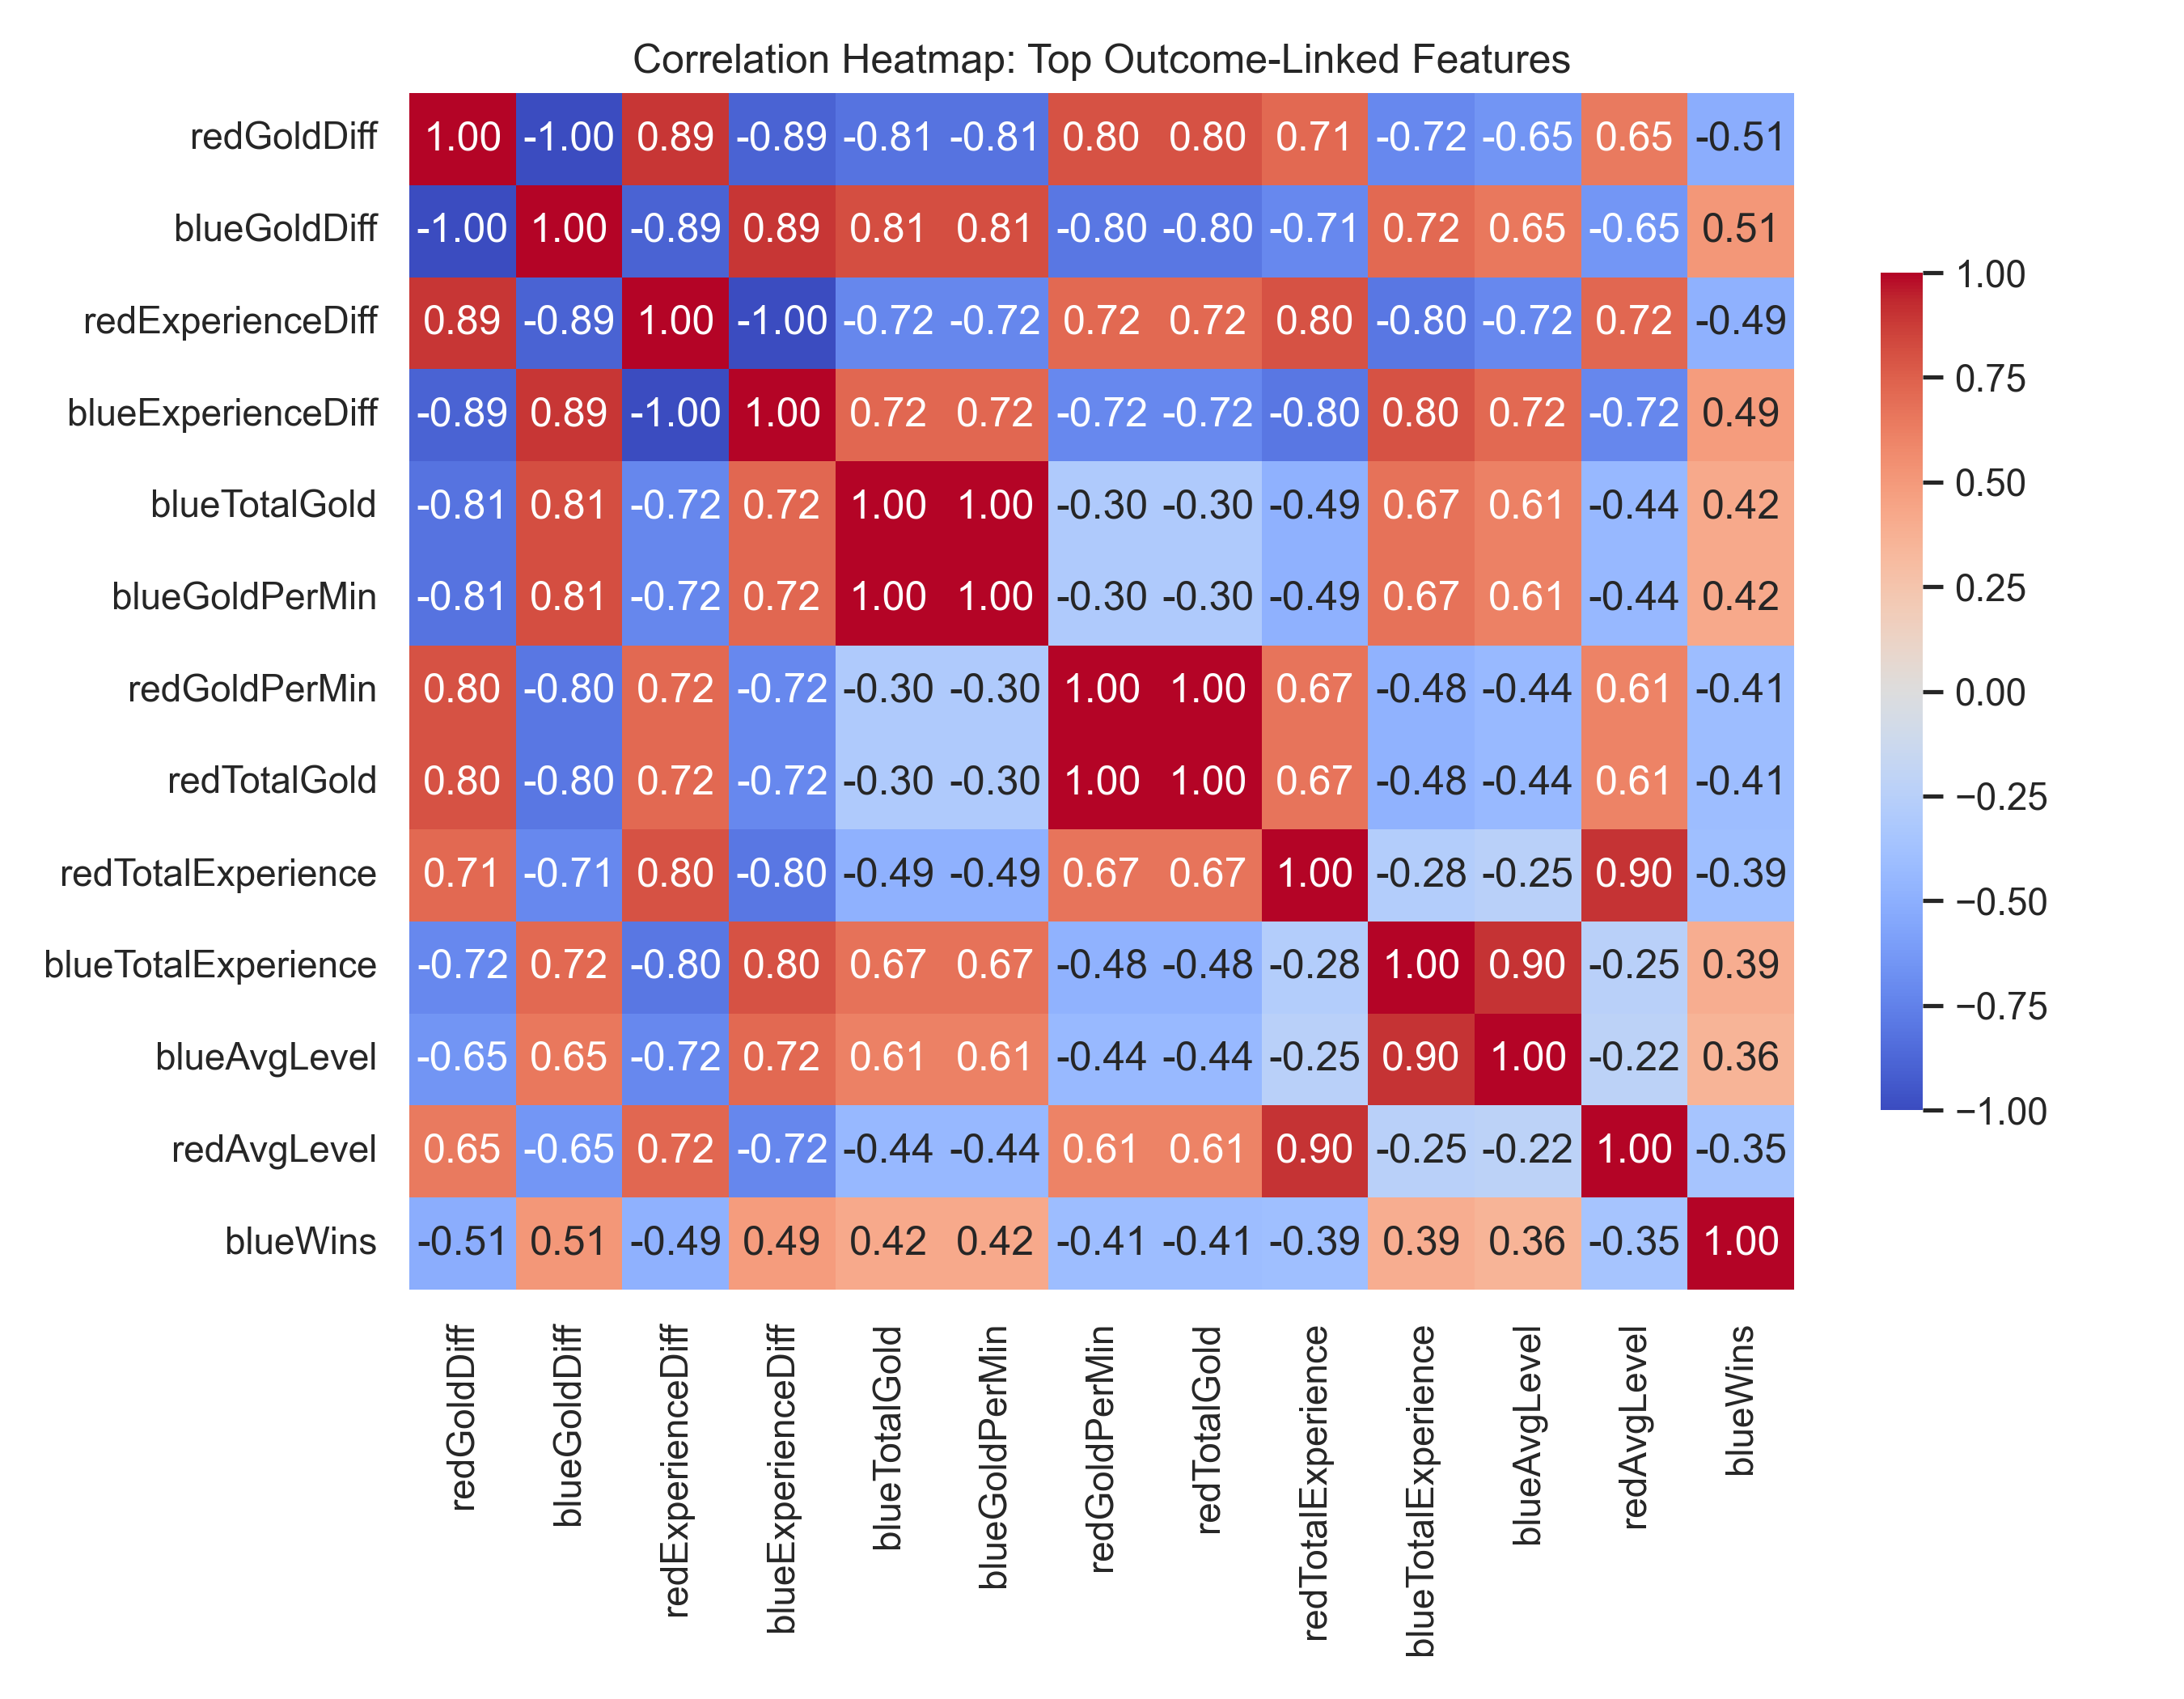
\includegraphics[width=0.8\linewidth]{figures/eda/top_feature_correlation_heatmap.png}
    \caption{Correlation structure among the twelve most outcome-sensitive features. Economic and experience signals dominate the predictive landscape.}
    \label{fig:heatmap}
\end{figure}

%%%%%%%%%%%%%%%%%%%%%%%%%%%%%%%%%%%%%%%%%%%%%%%%%%%%%%%%%%%%%%%%%%%%%%%%%%%%%%%
\section{Preprocessing}
\label{sec:preprocessing}
%%%%%%%%%%%%%%%%%%%%%%%%%%%%%%%%%%%%%%%%%%%%%%%%%%%%%%%%%%%%%%%%%%%%%%%%%%%%%%%

The preprocessing pipeline prioritizes reproducibility and leakage prevention. A dedicated Python script performs all steps and saves intermediates under version control.

\subsection{Data Splitting}
I perform an 80/20 stratified split on \texttt{blueWins} before any downstream analysis. Stratification ensures that both subsets mirror the global class balance, enabling fair model comparison and reliable baseline metrics. Split metadata (seed, counts, stratification flag) is persisted to \texttt{data/processed/split\_metadata.json}.

\subsection{Feature Engineering}
Initial experiments rely on the raw numeric telemetry. Planned feature engineering focuses on derived differentials (e.g., gold and experience deltas are already present), momentum ratios (CS per minute versus gold per minute), and aggregated objective indicators such as ``first dragon secured.'' Additional engineered features, such as smoothed rolling advantages or ward-efficiency ratios, will be explored if tree-based models expose overfitting to raw counts.

\subsection{Scaling, Transformation, and Encoding}
Because all predictors are numeric, preprocessing centers on scaling and optional log transformations. Linear models and neural networks will leverage a \texttt{StandardScaler} to normalize means and variances, whereas tree ensembles operate on the unscaled values. No categorical encoding or imputation is required given the dataset's completeness.

%%%%%%%%%%%%%%%%%%%%%%%%%%%%%%%%%%%%%%%%%%%%%%%%%%%%%%%%%%%%%%%%%%%%%%%%%%%%%%%
\section{Machine Learning Task and Objective}
\label{sec:ml_task}
%%%%%%%%%%%%%%%%%%%%%%%%%%%%%%%%%%%%%%%%%%%%%%%%%%%%%%%%%%%%%%%%%%%%%%%%%%%%%%%

This project tackles a supervised binary classification problem. The input features summarize both teams' performance during the first ten minutes, and the output predicts whether the Blue side ultimately wins. Traditional heuristics collapse multiple signals into hand-tuned weights, but they fail to capture nonlinear interactions, such as how simultaneous gold and objective advantages compound win probability. Machine learning models can ingest the full feature space and learn decision boundaries that align with historical outcomes, enabling accurate real-time forecasts and deeper analytic narratives.

%%%%%%%%%%%%%%%%%%%%%%%%%%%%%%%%%%%%%%%%%%%%%%%%%%%%%%%%%%%%%%%%%%%%%%%%%%%%%%%
\section{Models}
\label{sec:models}
%%%%%%%%%%%%%%%%%%%%%%%%%%%%%%%%%%%%%%%%%%%%%%%%%%%%%%%%%%%%%%%%%%%%%%%%%%%%%%%

I will benchmark three models that increase in flexibility and interpretability complexity.

\subsection{Model Selection}

\subsubsection{Model 1: Penalized Logistic Regression}
A logistic regression baseline, regularized with L2 penalty, offers transparent coefficients that quantify the marginal impact of each feature. Its simplicity provides a sanity check against the majority-class classifier and establishes lower bounds for accuracy, F1, and ROC-AUC.

\subsubsection{Model 2: Random Forest}
An ensemble of decision trees captures nonlinear thresholds and feature interactions without extensive preprocessing. I will tune the number of estimators, maximum depth, and minimum samples per split using stratified five-fold cross-validation. Variable importance scores from the fitted forest reveal the relative contribution of economic versus objective-based signals.

\subsubsection{Model 3: Multilayer Perceptron}
A compact multilayer perceptron (two hidden layers with dropout) can model smooth nonlinearities and feature synergies beyond axis-aligned splits. This architecture draws on prior esports prediction work \cite{liu2021ml}. Hyperparameters include hidden width, activation functions, dropout rate, and learning rate, optimized with validation folds.

\subsection{Regularization and Hyperparameter Tuning}
Grid searches will sweep penalty strengths for logistic regression, tree depths and estimators for the random forest, and optimizer settings for the neural network. I will rely on stratified five-fold cross-validation to estimate generalization performance and guard against overfitting. Early stopping based on validation loss will regulate the neural network.

%%%%%%%%%%%%%%%%%%%%%%%%%%%%%%%%%%%%%%%%%%%%%%%%%%%%%%%%%%%%%%%%%%%%%%%%%%%%%%%
\section{Training Methodology}
\label{sec:training}
%%%%%%%%%%%%%%%%%%%%%%%%%%%%%%%%%%%%%%%%%%%%%%%%%%%%%%%%%%%%%%%%%%%%%%%%%%%%%%%

\subsection{Loss Functions}
Logistic regression and the neural network optimize the binary cross-entropy loss,
\begin{equation}
\mathcal{L}(\theta) = -\frac{1}{n}\sum_{i=1}^{n} \left[y_i \log \hat{y}_i + (1 - y_i) \log (1 - \hat{y}_i)\right] + \lambda \|\theta\|_2^2,
\end{equation}
where $\hat{y}_i$ denotes the predicted win probability and $\lambda$ controls L2 regularization. The random forest minimizes impurity (Gini) at each split; its implicit loss corresponds to maximizing information gain across trees.

\subsection{Training Process}
Training proceeds in three phases: (1) compute baseline metrics on the holdout set using the logistic model to validate the pipeline, (2) perform cross-validated hyperparameter searches for each candidate model, and (3) refit the best configuration on the full training set before evaluating on the holdout split. I will log learning curves for the neural network and monitor validation AUC to trigger early stopping. For the random forest, out-of-bag error estimates provide an additional generalization check.

\subsection{Model Summary Table}

\begin{table}[H]
\centering
\caption{Planned models, tunable hyperparameters, and regularization strategies.}
\label{tab:model_summary}
\begin{tabular}{@{}lllll@{}}
\toprule
\textbf{Model} & \textbf{Key Parameters} & \textbf{Hyperparameters} & \textbf{Loss / Criterion} & \textbf{Regularization} \\ \midrule
Logistic Regression & Coefficients $\theta$ & $C \in \{0.01, 0.1, 1, 10\}$ & Binary cross-entropy & L2 penalty \\
Random Forest & Tree ensemble & Estimators, depth, min split & Gini impurity & Bootstrap averaging \\
Multilayer Perceptron & Layer weights & Hidden units, dropout, lr & Binary cross-entropy & Dropout, L2 weight decay \\
\bottomrule
\end{tabular}
\end{table}

%%%%%%%%%%%%%%%%%%%%%%%%%%%%%%%%%%%%%%%%%%%%%%%%%%%%%%%%%%%%%%%%%%%%%%%%%%%%%%%
\section{Metrics}
\label{sec:metrics}
%%%%%%%%%%%%%%%%%%%%%%%%%%%%%%%%%%%%%%%%%%%%%%%%%%%%%%%%%%%%%%%%%%%%%%%%%%%%%%%

Accuracy, F1 score, and ROC-AUC form the evaluation triad. Accuracy reports the percentage of correctly classified matches, F1 balances precision and recall for the positive class, and ROC-AUC captures ranking performance across thresholds.

\subsection{Primary Metric}
ROC-AUC will serve as the primary metric because production analysts care about ranking confidence---a model that scores actual winners higher than losers is valuable even if a single threshold is imperfect.

\subsection{Secondary Metrics}
Accuracy and F1 score quantify thresholded performance, with F1 emphasizing balanced sensitivity and precision when win/loss frequencies are comparable.

\subsection{Metric Definitions}
\begin{align}
\text{Accuracy} &= \frac{TP + TN}{TP + TN + FP + FN},\\
\text{F1} &= \frac{2 \cdot \text{Precision} \cdot \text{Recall}}{\text{Precision} + \text{Recall}},\\
\text{ROC-AUC} &= \int_{0}^{1} \text{TPR}(\text{FPR})\,d\text{FPR}.
\end{align}

%%%%%%%%%%%%%%%%%%%%%%%%%%%%%%%%%%%%%%%%%%%%%%%%%%%%%%%%%%%%%%%%%%%%%%%%%%%%%%%
\section{Results and Model Comparison}
\label{sec:results}
%%%%%%%%%%%%%%%%%%%%%%%%%%%%%%%%%%%%%%%%%%%%%%%%%%%%%%%%%%%%%%%%%%%%%%%%%%%%%%%

The baseline evaluation compares a majority-class dummy classifier with penalized logistic regression using the current preprocessing pipeline. Table~\ref{tab:baseline_performance} summarizes the metrics; improvements over the dummy model validate the feature set's predictive power. Future experiments will extend this table with random forest and neural network results and will log per-model training times to satisfy the final report requirements.

\begin{table}[H]
\centering
\caption{Baseline performance on the held-out test split.}
\label{tab:baseline_performance}
\begin{tabular}{@{}lccc@{}}
\toprule
\textbf{Model} & \textbf{Accuracy} & \textbf{F1} & \textbf{ROC-AUC} \\ \midrule
Dummy (Majority Class) & 0.50 & 0.00 & -- \\
Logistic Regression & 0.72 & 0.72 & 0.81 \\
\bottomrule
\end{tabular}
\end{table}

%%%%%%%%%%%%%%%%%%%%%%%%%%%%%%%%%%%%%%%%%%%%%%%%%%%%%%%%%%%%%%%%%%%%%%%%%%%%%%%
\section{Model Interpretation}
\label{sec:interpretation}
%%%%%%%%%%%%%%%%%%%%%%%%%%%%%%%%%%%%%%%%%%%%%%%%%%%%%%%%%%%%%%%%%%%%%%%%%%%%%%%

Interpretability is essential for communicating insights to analysts. For tree ensembles, I will compute permutation importance and SHAP values \cite{lundberg2017shap} to quantify how gold, experience, and objective metrics influence predictions. Logistic coefficients furnish readily interpretable odds ratios, while the neural network's attributions will be analyzed with Deep SHAP or integrated gradients if adopted. These diagnostics will feed into narrative explanations and help validate that the models align with established game knowledge.

%%%%%%%%%%%%%%%%%%%%%%%%%%%%%%%%%%%%%%%%%%%%%%%%%%%%%%%%%%%%%%%%%%%%%%%%%%%%%%%
\section{Conclusion}
\label{sec:conclusion}
%%%%%%%%%%%%%%%%%%%%%%%%%%%%%%%%%%%%%%%%%%%%%%%%%%%%%%%%%%%%%%%%%%%%%%%%%%%%%%%

\subsection{Summary of Findings}
Early experimentation confirms that ten-minute telemetry provides enough signal to beat naive baselines. Logistic regression already attains 0.81 ROC-AUC, indicating that economic and objective deltas are leading indicators of victory. The proposed experimentation plan will determine whether tree ensembles or shallow neural networks deliver further gains.

\subsection{Limitations and Future Work}
Current features omit draft compositions and player-specific tendencies that influence mid-game decisions. Future iterations could fuse champion picks, vision heatmaps, or time-series slices to capture tactical momentum. Additionally, calibrating predicted probabilities against actual win rates would improve trustworthiness for downstream decision-making.

\subsection{Final Remarks}
This proposal lays the groundwork for an interpretable, reproducible League of Legends win-probability model. Completing the planned experiments, interpretability analyses, and communication artifacts will satisfy the CMSE 492 final project requirements while producing insights valuable to the esports analytics community.

%%%%%%%%%%%%%%%%%%%%%%%%%%%%%%%%%%%%%%%%%%%%%%%%%%%%%%%%%%%%%%%%%%%%%%%%%%%%%%%
\section{Timeline and Milestones}
\label{sec:timeline}
%%%%%%%%%%%%%%%%%%%%%%%%%%%%%%%%%%%%%%%%%%%%%%%%%%%%%%%%%%%%%%%%%%%%%%%%%%%%%%%

Figure~\ref{fig:gantt} presents the project timeline spanning October 20 through December 8, 2025. Critical path tasks include exploratory analysis, feature engineering, and model benchmarking, with report writing and presentation preparation overlapping the final two weeks. Buffer time is reserved during Thanksgiving week for unexpected modeling setbacks or LaTeX revisions.

\begin{figure}[H]
    \centering
    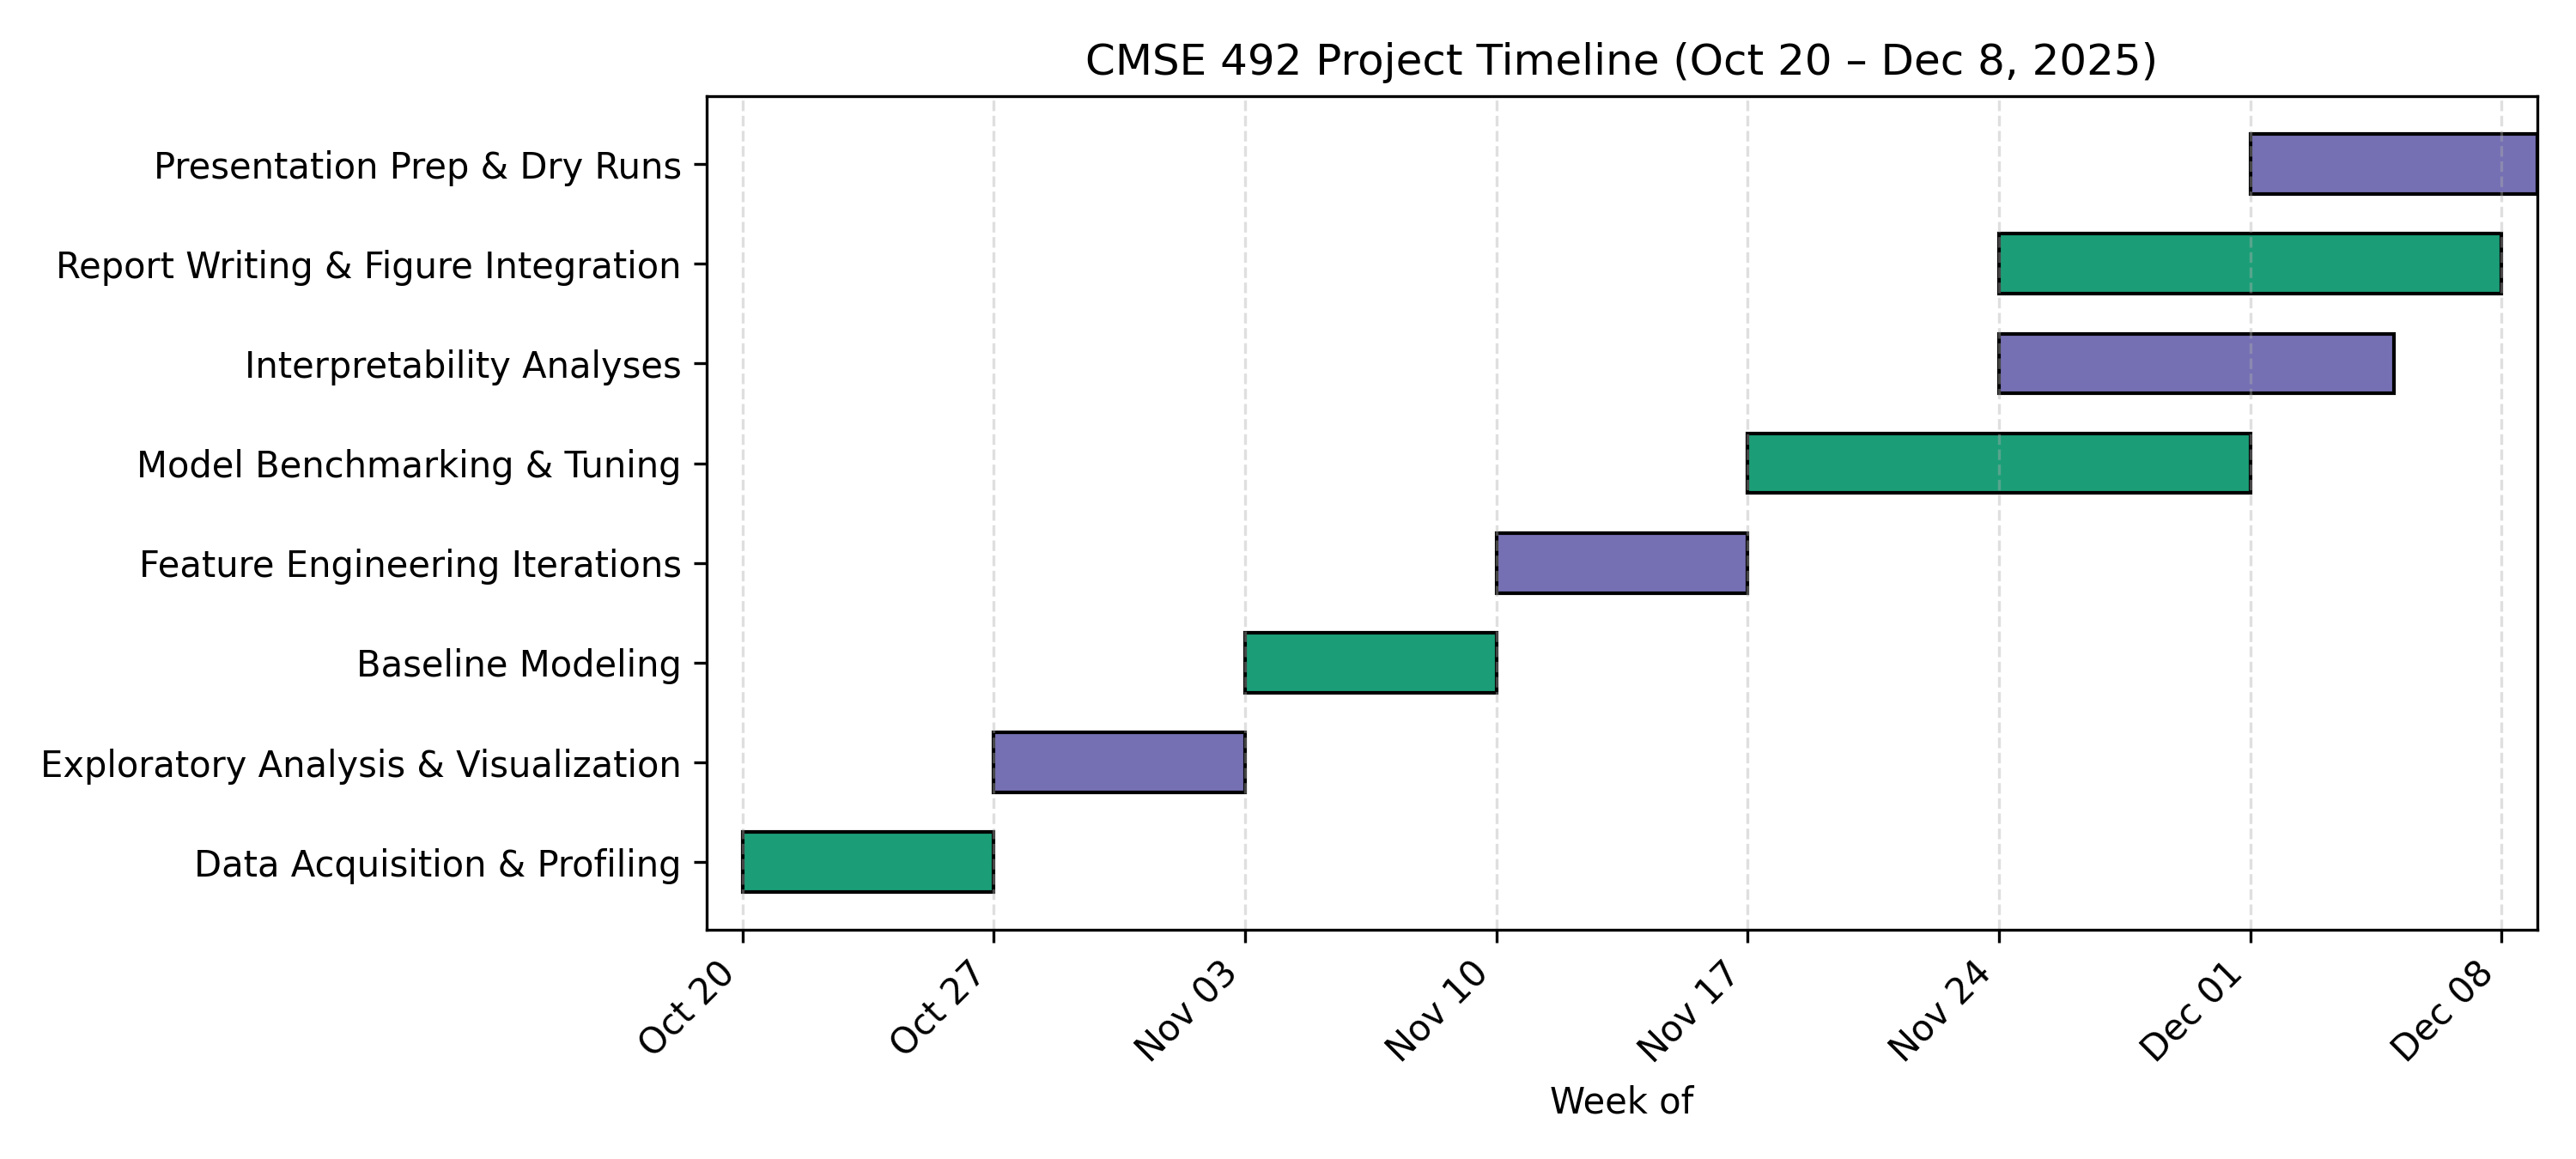
\includegraphics[width=0.85\linewidth]{figures/project_timeline.png}
    \caption{Project Gantt chart covering major milestones and deliverables.}
    \label{fig:gantt}
\end{figure}

%%%%%%%%%%%%%%%%%%%%%%%%%%%%%%%%%%%%%%%%%%%%%%%%%%%%%%%%%%%%%%%%%%%%%%%%%%%%%%%
\begin{acknowledgments}
I thank the CMSE 492 instructional team for curating the datasets and templates that scaffold this project.
\end{acknowledgments}

%%%%%%%%%%%%%%%%%%%%%%%%%%%%%%%%%%%%%%%%%%%%%%%%%%%%%%%%%%%%%%%%%%%%%%%%%%%%%%%
\begin{thebibliography}{99}

\bibitem{bobby2020lol}
B. De la Iglesia, ``League of Legends Diamond Ranked Games (10 min),'' Kaggle, 2020. Available at: \url{https://www.kaggle.com/datasets/bobbyscience/league-of-legends-diamond-ranked-games-10-min}.

\bibitem{lundberg2017shap}
S. M. Lundberg and S.-I. Lee, ``A Unified Approach to Interpreting Model Predictions,'' in \textit{Advances in Neural Information Processing Systems}, 2017.

\bibitem{liu2021ml}
T. Liu and Y. Wu, ``Predicting Match Outcomes in Esports Using Machine Learning,'' \textit{IEEE Transactions on Games}, vol. 13, no. 3, pp. 1--12, 2021.

\end{thebibliography}

\end{document}
